\documentclass[12pt,a4paper]{article}
\usepackage[utf8]{vietnam}
\usepackage{amsmath,amssymb}
\usepackage{geometry}
\geometry{top=1.5cm,bottom=1.2cm,left=1.4cm,right=1.4cm,headheight=28pt,headsep=12pt,footskip=18pt}
\usepackage{tikz}
\usepackage{xcolor}
\usepackage{enumerate}
\usepackage{graphicx}
\usepackage[version=4]{mhchem}
\usepackage{fancyhdr}
\usepackage{ex_test}

\renewcommand{\baselinestretch}{0.96}
\setlength{\parskip}{0pt}

\definecolor{hfRed}{RGB}{211,47,47}
\definecolor{hfGreen}{RGB}{139,195,144}

\pagestyle{fancy}
\fancyhf{}
\fancyhead[L]{\small\itshape\color{hfRed} Tài liệu lưu hành nội bộ}
\fancyhead[R]{\small\itshape\color{hfRed} Thầy \textbf{TRẦN VĂN THẠNH} - 0777.470.803}
\renewcommand{\headrulewidth}{0.8pt}
\renewcommand{\headrule}{\hbox to\headwidth{\color{hfGreen}\leaders\hrule height \headrulewidth\hfill}}

\fancyfoot[L]{\small\itshape\color{hfRed} CS1: 6/15 Nguyễn Hoàng, P. Kim Long, TP Huế \quad|\quad CS2: 24 Đặng Thái Thân, TP Huế}
\fancyfoot[R]{\small\bfseries\color{hfRed} Trang \thepage}
\renewcommand{\footrulewidth}{0.8pt}
\renewcommand{\footrule}{\hbox to\headwidth{\color{hfGreen}\leaders\hrule height \footrulewidth\hfill}}

\fancypagestyle{firstpage}{
  \fancyhf{}
  \renewcommand{\headrulewidth}{0pt}
  \fancyfoot[L]{\small\itshape\color{hfRed} CS1: 6/15 Nguyễn Hoàng, P. Kim Long, TP Huế \quad|\quad CS2: 24 Đặng Thái Thân, TP Huế}
  \fancyfoot[R]{\small\bfseries\color{hfRed} Trang \thepage}
  \renewcommand{\footrulewidth}{0.8pt}
  \renewcommand{\footrule}{\hbox to\headwidth{\color{hfGreen}\leaders\hrule height \footrulewidth\hfill}}
}

\begin{document}
\thispagestyle{firstpage}

\noindent
\begin{minipage}[t]{0.44\textwidth}
	\centering\fontsize{10pt}{12pt}\selectfont
	\textbf{SỞ GIÁO DỤC VÀ ĐÀO TẠO THỪA THIÊN HUẾ}\\
	\textbf{ĐỀ CHÍNH THỨC}\\
	\textit{(Đề thi có 04 trang)}
\end{minipage}\hfill
\begin{minipage}[t]{0.54\textwidth}
	\centering\fontsize{10.5pt}{13pt}\selectfont
	\textbf{ĐỀ KIỂM TRA ĐỊNH KỲ CHƯƠNG 5}\\
	\textbf{(DẪN XUẤT HALOGEN - ALCOHOL - PHENOL)}\\
	\textbf{MÔN: HOÁ HỌC - LỚP 11}\\
	\textit{Thời gian làm bài: 50 phút, không kể thời gian phát đề}
	
	\smallskip
	\fbox{\textbf{MÃ ĐỀ: 114}}
\end{minipage}

\smallskip
\begin{center}
	{\color{hfRed}\textbf{\large (BẢN GIÁO VIÊN -- CÓ LỜI GIẢI CHI TIẾT)}}
\end{center}

\smallskip
\noindent\hrulefill
\smallskip

\noindent\textbf{Họ, tên thí sinh:} \dotfill\ \textbf{Lớp:} \dotfill\ \textbf{Số báo danh:} \dotfill

\smallskip
\noindent\textit{(Cho biết nguyên tử khối: H = 1; C = 12; N = 14; O = 16; F = 19; Na = 23; Mg = 24; Al = 27; P = 31; S = 32; Cl = 35,5; K = 39; Ca = 40; Cr = 52; Mn = 55; Fe = 56; Cu = 64; Zn = 65; Br = 80; Ag = 108; I = 127).}
\smallskip

\noindent\textbf{\large PHẦN I. Câu trắc nghiệm nhiều phương án lựa chọn.}
\textit{Thí sinh trả lời từ câu 1 đến câu 18. Mỗi câu hỏi thí sinh chỉ chọn một phương án.}
\vspace{0.2cm}

\Opensolutionfile{ans}[ans-hoa11-de14gv]

% Câu 1
\begin{ex}
Chất nào \textbf{không} phải là dẫn xuất halogen của hydrocarbon?
\choice
{\ce{CH2=CH-CH2Br}}
{\ce{ClBrCH-CF3}}
{\True \ce{Cl2CH-CF2-O-CH3}}
{\ce{C6H6Cl6}}
\loigiai{
Dẫn xuất halogen của hydrocarbon chỉ được cấu tạo từ các nguyên tố C, H và halogen (F, Cl, Br, I). Chất C (\ce{Cl2CH-CF2-O-CH3}) chứa thêm nguyên tố O nên là một ether chứa halogen, không phải dẫn xuất halogen của hydrocarbon.
}
\end{ex}

% Câu 2
\begin{ex}
Dẫn xuất halogen nào sau đây \textbf{không} có đồng phân cis-trans?
\choice
{\ce{CHCl=CHCl}}
{\True \ce{CH2=CH-CH2F}}
{\ce{CH3CH=CBrCH3}}
{\ce{CH3CH2CH=CHCHClCH3}}
\loigiai{
Điều kiện để có đồng phân hình học cis-trans là mỗi nguyên tử carbon mang liên kết đôi phải liên kết với hai nhóm nguyên tử khác nhau ($R_1 \ne R_2$ và $R_3 \ne R_4$). Chất B có nhóm đầu mạch \ce{CH2=} chứa 2 nguyên tử H giống nhau nên không có đồng phân cis-trans.
}
\end{ex}

% Câu 3
\begin{ex}
Chloromethane, còn được gọi với những cái tên khác là methyl chloride, Refrigerant-40, R-40 hoặc HCC 40, là một hợp chất hóa học thuộc nhóm haloalkane. Nó từng được sử dụng rộng rãi như một chất làm lạnh. Công thức phân tử của chloromethane là
\choice
{\ce{CH2Cl2}}
{\True \ce{CH3Cl}}
{\ce{CHCl3}}
{\ce{CCl4}}
\loigiai{
Chloromethane (methyl chloride) có công thức phân tử là \ce{CH3Cl}.
}
\end{ex}

% Câu 4
\begin{ex}
Nhiệt độ nóng chảy, nhiệt độ sôi của alcohol đều cao hơn so với hydrocarbon, dẫn xuất halogen, ether có phân tử lượng tương đương là do
\choice
{trong phân tử alcohol có liên kết cộng hoá trị}
{\True giữa các phân tử alcohol có liên kết hydrogen liên phân tử}
{alcohol có nguyên tử oxygen trong phân tử}
{alcohol có phản ứng với Na}
\loigiai{
Giữa các phân tử alcohol có khả năng tạo liên kết hydrogen liên phân tử bền vững, làm cho các phân tử liên kết chặt chẽ hơn với nhau, do đó cần nhiều năng lượng hơn để phá vỡ nên nhiệt độ sôi và nhiệt độ nóng chảy của alcohol cao hơn nhiều so với hydrocarbon, dẫn xuất halogen, ether có phân tử lượng tương đương.
}
\end{ex}

% Câu 5
\begin{ex}
Alcohol nào sau đây khi bị oxi hóa bởi \ce{CuO} ($t^\circ$) tạo acetone?
\choice
{\True propan-2-ol}
{butan-1-ol}
{2-methylpropan-1-ol}
{propan-1-ol}
\loigiai{
Khi bị oxi hóa không hoàn toàn bởi \ce{CuO} nung nóng, alcohol bậc II bị oxi hóa tạo ketone. Propan-2-ol (\ce{CH3CH(OH)CH3}) là alcohol bậc II tạo ra acetone (\ce{CH3COCH3}):\\
\ce{CH3CH(OH)CH3 + CuO ->[{t$^\circ$}] CH3COCH3 + Cu + H2O}.
}
\end{ex}

% Câu 6
\begin{ex}
Khi đun nóng dẫn xuất halogen X với dung dịch \ce{NaOH} tạo thành hợp chất acetic aldehyde. Tên của hợp chất X là
\choice
{1,2-dibromoethane}
{\True 1,1-dibromoethane}
{ethyl chloride}
{A và B đúng}
\loigiai{
Phương trình: \ce{CH3CHBr2 + 2NaOH ->[{t$^\circ$}] CH3CHO + 2NaBr + H2O}.\\
Hợp chất gem-dihalide có hai nguyên tử halogen gắn vào cùng một nguyên tử carbon đầu mạch khi thủy phân sẽ tạo aldehyde. Hợp chất X là 1,1-dibromoethane (\ce{CH3CHBr2}).
}
\end{ex}

% Câu 7
\begin{ex}
Tên gọi theo danh pháp thay thế của alcohol \ce{(CH3)2CHCH2CH2OH} là
\choice
{2-methylbutan-1-ol}
{\True 3-methylbutan-1-ol}
{3-methylbutan-2-ol}
{1,1-dimethylpropan-2-ol}
\loigiai{
Đánh số mạch chính từ phía gần nhóm \ce{-OH} nhất:
$\overset{4}{\text{C}}\text{H}_3 - \overset{3}{\text{C}}\text{H}(\text{CH}_3) - \overset{2}{\text{C}}\text{H}_2 - \overset{1}{\text{C}}\text{H}_2\text{OH}$.\\
Nhóm methyl ở vị trí C số 3, nhóm \ce{-OH} ở vị trí C số 1 $\Rightarrow$ Tên thay thế: 3-methylbutan-1-ol.
}
\end{ex}

% Câu 8
\begin{ex}
Tên thay thế của alcohol có công thức cấu tạo thu gọn \ce{CH3CH2CH2OH} là
\choice
{\True propan-1-ol}
{propan-2-ol}
{pentan-1-ol}
{pentan-2-ol}
\loigiai{
Mạch chính có 3 carbon no, nhóm \ce{-OH} ở vị trí số 1 nên tên thay thế là propan-1-ol.
}
\end{ex}

% Câu 9
\begin{ex}
Catechin là chất chống oxi hoá mạnh có trong lá chè tươi và nhiều loại quả, có khả năng phòng chống ung thư và tim mạch. Công thức cấu tạo của catechin được cho như hình bên:
\begin{center}
	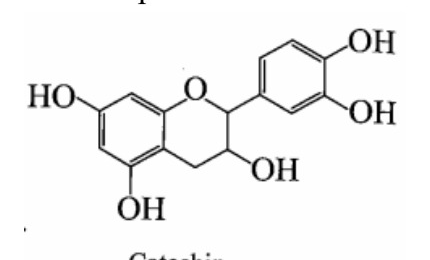
\includegraphics[width=0.42\textwidth]{images_crop_hoa11_de14/catechin_structure.png}
\end{center}
Phát biểu nào sau đây \textbf{không đúng}?
\choice
{Công thức phân tử của catechin là \ce{C15H14O6}}
{\True Phân tử catechin có 5 nhóm OH phenol}
{Catechin phản ứng được với dung dịch \ce{NaOH}}
{Catechin thuộc loại hợp chất thơm}
\loigiai{
Quan sát công thức cấu tạo của catechin:
\begin{itemize}
    \item Có 4 nhóm \ce{-OH} gắn trực tiếp vào vòng benzene (thuộc loại nhóm OH phenol): 2 nhóm ở vòng A và 2 nhóm ở vòng B.
    \item Có 1 nhóm \ce{-OH} gắn vào carbon no của dị vòng chứa O (thuộc loại nhóm OH alcohol).
\end{itemize}
Do đó, phân tử catechin chỉ có 4 nhóm OH phenol và 1 nhóm OH alcohol (không phải 5 nhóm OH phenol).\\
Công thức phân tử là \ce{C15H14O6}. Do có nhóm OH phenol nên phản ứng được với dung dịch \ce{NaOH}; phân tử chứa vòng benzene nên là hợp chất thơm.
}
\end{ex}

% Câu 10
\begin{ex}
Trong thực tế, phenol được dùng làm nguyên liệu để sản xuất
\choice
{nhựa poly(vinyl chloride), nhựa novolac và chất diệt cỏ 2,4-D}
{nhựa resol, nhựa resit và thuốc trừ sâu 666}
{\True poly(phenol-formaldehyde), chất diệt cỏ 2,4-D và picric acid}
{nhựa resit, chất diệt cỏ 2,4-D và thuốc nổ TNT}
\loigiai{
Phenol là nguyên liệu quan trọng trong công nghiệp hóa chất để sản xuất nhựa poly(phenol - formaldehyde) (novolac, resol), chất diệt cỏ 2,4-D (2,4-dichlorophenoxyacetic acid) và chất nổ picric acid (2,4,6-trinitrophenol).
}
\end{ex}

% Câu 11
\begin{ex}
Để chứng minh sự ảnh hưởng qua lại của nhóm \ce{-OH} và vòng benzene trong phenol (\ce{C6H5OH}) thì cần cho phenol tác dụng với các chất nào sau đây?
\choice
{Na và nước \ce{Br2}}
{Dung dịch \ce{NaOH} và khí \ce{CO2}}
{\True Dung dịch \ce{NaOH} và nước \ce{Br2}}
{Quỳ tím và nước \ce{Br2}}
\loigiai{
- Ảnh hưởng của vòng benzene lên nhóm \ce{-OH}: Làm tăng độ phân cực của liên kết O-H, phenol có tính acid yếu, phản ứng được với dung dịch \ce{NaOH} (trong khi alcohol không phản ứng).\\
- Ảnh hưởng của nhóm \ce{-OH} lên vòng benzene: Hoạt hóa các vị trí \textit{ortho} và \textit{para} của vòng thơm, làm phenol phản ứng dễ dàng với dung dịch nước bromine (\ce{Br2}) tạo kết tủa trắng 2,4,6-tribromophenol (trong khi benzene không phản ứng ở điều kiện này).\\
Do đó cần dùng dung dịch \ce{NaOH} và nước \ce{Br2}.
}
\end{ex}

% Câu 12
\begin{ex}
Hiện tượng xảy ra khi nhỏ vài giọt dung dịch \ce{HCl} đặc vào ống nghiệm chứa một ít dung dịch \ce{C6H5ONa} rồi lắc mạnh là
\choice
{có sự phân lớp; dung dịch trong suốt hóa đục}
{\True dung dịch trong suốt hóa đục}
{có phân lớp; dung dịch trong suốt}
{xuất hiện sự phân lớp ở ống nghiệm}
\loigiai{
Phương trình: \ce{C6H5ONa + HCl -> C6H5OH v + NaCl}.\\
Phenol sinh ra rất ít tan trong nước lạnh ở điều kiện thường nên làm cho dung dịch từ trong suốt chuyển sang hóa đục.
}
\end{ex}

% Câu 13
\begin{ex}
Sản phẩm chính tạo thành khi cho 2-bromobutane tác dụng với dung dịch \ce{KOH} trong ethanol, đun nóng là
\choice
{methylcyclopropane}
{but-2-ol}
{but-1-ene}
{\True but-2-ene}
\loigiai{
Theo quy tắc tách Zaitsev, khi tách hydrogen halide khỏi dẫn xuất halogen, nguyên tử halogen bị tách ưu tiên cùng với nguyên tử H ở carbon bậc cao hơn bên cạnh để tạo alkene có nhiều nhóm thế hơn (bền hơn):\\
\ce{CH3-CHBr-CH2-CH3 + KOH ->[{C_2H_5OH, t$^\circ$}] CH3-CH=CH-CH3} (sp chính: but-2-ene) \ce{+ KBr + H2O}.
}
\end{ex}

% Câu 14
\begin{ex}
(SBT-KNTT) Sản phẩm chính thu được khi tách nước từ 3-methylbutan-2-ol là
\choice
{3-methylbut-1-ene}
{\True 2-methylbut-2-ene}
{3-methylbut-2-ene}
{2-methylbut-3-ene}
\loigiai{
Tách nước từ 3-methylbutan-2-ol: \ce{CH3-CH(CH3)-CH(OH)-CH3 ->[{H_2SO_4, t$^\circ$}]}\\
- Tách H cùng carbon bậc cao hơn (C số 3 là carbon bậc III có 1 H) theo quy tắc Zaitsev tạo sản phẩm chính: \ce{CH3-C(CH3)=CH-CH3} (2-methylbut-2-ene).\\
- Tách H ở C số 1 tạo sản phẩm phụ: \ce{CH3-CH(CH3)-CH=CH2} (3-methylbut-1-ene).
}
\end{ex}

% Câu 15
\begin{ex}
(SBT-KNTT) Oxi hoá alcohol nào sau đây thu được sản phẩm là ketone?
\choice
{\ce{C2H5OH}}
{\ce{CH3CH2CH2OH}}
{\True \ce{CH3CH(OH)CH3}}
{\ce{(CH3)2C(OH)CH3}}
\loigiai{
Oxi hóa alcohol bậc II bằng \ce{CuO} nung nóng thu được ketone:\\
\ce{CH3-CH(OH)-CH3 + CuO ->[{t$^\circ$}] CH3-CO-CH3 + Cu + H2O}.\\
Chất C là propan-2-ol (isopropyl alcohol) tạo acetone. (A và B là alcohol bậc I cho aldehyde; D là alcohol bậc III không bị oxi hóa trong điều kiện này).
}
\end{ex}

% Câu 16
\begin{ex}
Cho các phát biểu sau:
\begin{enumerate}[(1)]
    \item Phenol tan vô hạn trong nước ở 66\,$^\circ$C.
    \item Phenol có lực acid mạnh hơn alcohol ethylic.
    \item Phản ứng thế vào benzene dễ hơn phản ứng thế vào nhân thơm của phenol.
    \item Phenol tan tốt trong ethanol.
    \item Phenol làm quỳ tím hóa đỏ.
    \item Nhóm OH phenol không bị thế bởi gốc acid như nhóm OH alcohol.
\end{enumerate}
Có bao nhiêu phát biểu đúng?
\choice
{5}
{\True 4}
{3}
{6}
\loigiai{
(1) Đúng. Phenol ít tan trong nước lạnh nhưng tan vô hạn trong nước ở nhiệt độ trên 66\,$^\circ$C.\\
(2) Đúng. Do vòng benzene hút electron làm tăng độ phân cực của liên kết O-H nên phenol có tính acid mạnh hơn alcohol ethylic.\\
(3) Sai. Nhóm \ce{-OH} đẩy electron vào vòng benzene làm tăng mật độ electron của vòng thơm nên phản ứng thế vào nhân thơm của phenol dễ hơn nhiều so với benzene.\\
(4) Đúng. Phenol tan tốt trong các dung môi hữu cơ như ethanol, ether,...\\
(5) Sai. Phenol có tính acid rất yếu (yếu hơn carbonic acid \ce{H2CO3}) nên không làm đổi màu quỳ tím.\\
(6) Đúng. Nhóm \ce{-OH} phenol liên kết trực tiếp với vòng thơm có hiệu ứng liên hợp $p-\pi$, liên kết C-O rất bền vững nên nhóm \ce{-OH} không bị thế bởi gốc acid như trong phản ứng ester hóa thông thường của alcohol.\\
$\Rightarrow$ Có 4 phát biểu đúng là (1), (2), (4), (6).
}
\end{ex}

% Câu 17
\begin{ex}
X là hỗn hợp gồm hai alkene (ở thể khí trong điều kiện thường). Hydrate hóa X được hỗn hợp Y gồm 4 alcohol (không có alcohol bậc III). X gồm
\choice
{\True propene và but-1-ene}
{ethylene và propene}
{propene và but-2-ene}
{propene và 2-methylpropene}
\loigiai{
- Hai alkene ở thể khí trong điều kiện thường: Có số nguyên tử C $\le 4$.\\
- Hỗn hợp Y gồm 4 alcohol và không có alcohol bậc III.\\
Xét các phương án:
\begin{itemize}
    \item A. Propene (\ce{CH2=CH-CH3}) hydrate hóa tạo 2 alcohol: propan-1-ol (bậc I) và propan-2-ol (bậc II). But-1-ene (\ce{CH2=CH-CH2-CH3}) hydrate hóa tạo 2 alcohol: butan-1-ol (bậc I) và butan-2-ol (bậc II). Cả 4 alcohol này đều khác nhau và đều là bậc I hoặc bậc II (không có bậc III). Thỏa mãn.
    \item B. Ethylene chỉ tạo 1 alcohol (\ce{C2H5OH}), propene tạo 2 alcohol $\Rightarrow$ tổng cộng 3 alcohol (loại).
    \item C. But-2-ene đối xứng chỉ tạo 1 alcohol (butan-2-ol), propene tạo 2 alcohol $\Rightarrow$ tổng cộng 3 alcohol (loại).
    \item D. 2-methylpropene hydrate hóa tạo 2-methylpropan-2-ol là alcohol bậc III (loại).
\end{itemize}
}
\end{ex}

% Câu 18
\begin{ex}
Nghiên cứu số liệu về năng lượng liên kết, độ dài liên kết và độ phân cực carbon - halogen:
\begin{center}
\begin{tabular}{|l|c|c|c|c|}
\hline
\textbf{Đặc điểm} & \textbf{C-F} & \textbf{C-Cl} & \textbf{C-Br} & \textbf{C-I} \\
\hline
Năng lượng liên kết (kJ/mol) & 453 & 339 & 276 & 216 \\
\hline
Độ dài liên kết (pm) & 133 & 177 & 194 & 213 \\
\hline
\end{tabular}
\end{center}
\begin{center}
	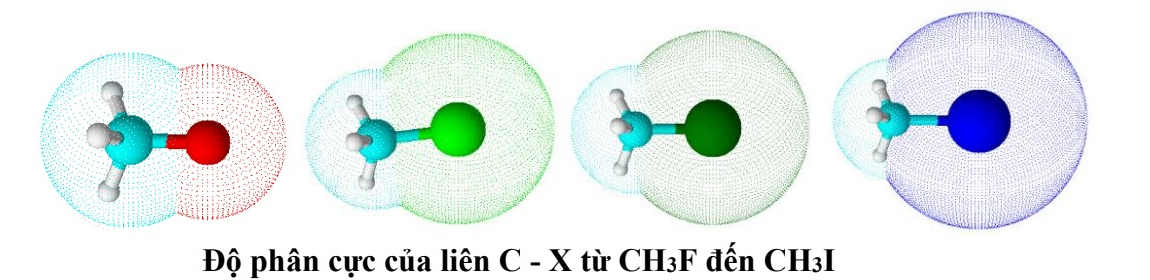
\includegraphics[width=0.65\textwidth]{images_crop_hoa11_de14/cx_polarity.png}
\end{center}
Khả năng phản ứng thế nguyên tử halogen bằng nhóm \ce{-OH} tăng theo chiều nào sau đây?
\choice
{\True \ce{C-F < C-Cl < C-Br < C-I}}
{\ce{C-I < C-Cl < C-Br < C-F}}
{\ce{C-F < C-Br < C-Cl < C-I}}
{\ce{C-I < C-Br < C-Cl < C-F}}
\loigiai{
Từ C-F đến C-I: Năng lượng liên kết C-X giảm dần (từ 453 xuống 216 kJ/mol), độ dài liên kết tăng dần (từ 133 lên 213 pm), liên kết C-X trở nên kém bền hơn và dễ bị phân cắt hơn. Đồng thời độ phân cực giảm dần làm giảm lực hút tĩnh điện giữa C và X. Do đó, khả năng phản ứng thế nguyên tử halogen bằng nhóm \ce{-OH} tăng dần theo chiều: \ce{C-F < C-Cl < C-Br < C-I}.
}
\end{ex}

\Closesolutionfile{ans}

\bigskip
\noindent\textbf{\large PHẦN II. Câu trắc nghiệm đúng sai.}
\textit{Thí sinh trả lời từ câu 1 đến câu 4. Trong mỗi ý a), b), c), d) ở mỗi câu, thí sinh chọn đúng hoặc sai.}
\vspace{0.2cm}

% Câu 1 Phần II
\begin{ex}
Danh pháp và cấu tạo của dẫn xuất halogen.\\
Trong thực tế sản xuất, methyl chloride (\ce{CH3Cl}) được sử dụng rộng rãi trong công nghiệp. Hãy xác định đúng/sai cho các mệnh đề sau:
\choiceTF
{\True Methyl chloride thuộc nhóm dẫn xuất halogen}
{\True Công thức cấu tạo của methyl chloride là \ce{CH3Cl}, trong đó nguyên tử Cl liên kết với nguyên tử C}
{Theo danh pháp thay thế, \ce{CH3Cl} được gọi là chloroethane}
{\True Methyl chloride là một hợp chất khí dễ bay hơi, có thể gây nguy hiểm khi hít phải trong thời gian dài}
\loigiai{
- a) ĐÚNG: \ce{CH3Cl} được tạo thành khi thay thế 1 nguyên tử H của methane bằng 1 nguyên tử Cl, thuộc nhóm dẫn xuất halogen.\\
- b) ĐÚNG: Nguyên tử carbon liên kết trực tiếp với 3 nguyên tử H và 1 nguyên tử Cl.\\
- c) SAI: Theo danh pháp thay thế, \ce{CH3Cl} có tên là chloromethane (không phải chloroethane).\\
- d) ĐÚNG: Methyl chloride là chất khí không màu, dễ bay hơi, độc hại khi hít phải trong thời gian dài, gây ức chế thần kinh trung ương.
}
\end{ex}

% Câu 2 Phần II
\begin{ex}
Hợp chất X có tác dụng kháng khuẩn, chống vi sinh vật kí sinh trên da (chấy, rận,...). X có công thức phân tử \ce{C7H8O} và có chứa vòng benzene, phổ IR của X có peak hấp thụ rộng ở vùng 3\,300 $\text{cm}^{-1}$. Oxi hóa X bằng \ce{CuO} nung nóng, thu được hợp chất Y có peak hấp thụ đặc trưng ở khoảng 1\,700 $\text{cm}^{-1}$.
\choiceTF
{Phổ IR của X có peak hấp thụ rộng ở vùng 3\,300 $\text{cm}^{-1}$ nên X có nhóm C=O}
{Phổ IR của Y có peak hấp thụ rộng ở vùng 1\,700 $\text{cm}^{-1}$ nên Y có nhóm \ce{-OH}}
{\True X là benzyl alcohol, Y là aldehyde benzoic}
{Y tan nhiều trong nước hơn X}
\loigiai{
- a) SAI: Peak hấp thụ rộng ở vùng $3\,200 - 3\,600\,\text{cm}^{-1}$ đặc trưng cho liên kết O-H (alcohol hoặc phenol), không phải C=O.\\
- b) SAI: Peak hấp thụ mạnh ở khoảng $1\,700\,\text{cm}^{-1}$ đặc trưng cho nhóm carbonyl C=O (aldehyde hoặc ketone), không phải \ce{-OH}.\\
- c) ĐÚNG: X chứa vòng benzene, công thức \ce{C7H8O}, có nhóm \ce{-OH} và bị oxi hóa bởi \ce{CuO} tạo aldehyde Y nên X là alcohol bậc I: benzyl alcohol (\ce{C6H5CH2OH}), và Y là benzaldehyde (aldehyde benzoic, \ce{C6H5CHO}).\\
- d) SAI: Cả X và Y đều chứa gốc phenyl kỵ nước lớn nên ít tan trong nước, nhưng benzyl alcohol (X) tạo được liên kết hydrogen với phân tử nước nên độ tan trong nước của X lớn hơn so với benzaldehyde (Y).
}
\end{ex}

% Câu 3 Phần II
\begin{ex}
Thực hiện thí nghiệm copper(II) hydroxide tác dụng với alcohol đa chức:\\
\textit{Bước 1:} Cho vào ống nghiệm 1 mL dung dịch \ce{CuSO4} 2\% và 1 mL dung dịch \ce{NaOH} 10\%.\\
\textit{Bước 2:} Lắc nhẹ ống nghiệm rồi nhỏ vào 5 giọt glycerol.\\
- Sau bước 1, thấy xuất hiện kết tủa xanh lơ trong ống nghiệm.\\
- Sau bước 2, kết tủa tan thành dung dịch xanh lam đậm.
\choiceTF
{\True Thí nghiệm chứng tỏ glycerol có các nhóm OH liền kề}
{Nếu thay glycerol bằng ethanol, hiện tượng vẫn tương tự}
{\True Có thể dùng thí nghiệm này để nhận biết glycerol và ethanol}
{Không thể dùng \ce{Cu(OH)2} để nhận biết methanol và ethylene glycol}
\loigiai{
- a) ĐÚNG: Phản ứng hòa tan kết tủa \ce{Cu(OH)2} tạo dung dịch phức màu xanh lam đậm đặc trưng cho polyalcohol có ít nhất hai nhóm \ce{-OH} liền kề (như glycerol, ethylene glycol).\\
- b) SAI: Ethanol là alcohol đơn chức, không có khả năng tạo phức hòa tan \ce{Cu(OH)2}, kết tủa xanh không tan.\\
- c) ĐÚNG: Glycerol hòa tan \ce{Cu(OH)2} tạo dung dịch màu xanh lam đậm, còn ethanol không hòa tan \ce{Cu(OH)2}.\\
- d) SAI: Hoàn toàn có thể dùng \ce{Cu(OH)2} để nhận biết methanol và ethylene glycol vì ethylene glycol hòa tan \ce{Cu(OH)2} tạo dung dịch màu xanh lam đậm, còn methanol không có hiện tượng.
}
\end{ex}

% Câu 4 Phần II
\begin{ex}
Eugenol là thành phần chính của tinh dầu hương nhu có công thức phân tử \ce{C10H12O2}. Eugenol có công thức cấu tạo:
\begin{center}
	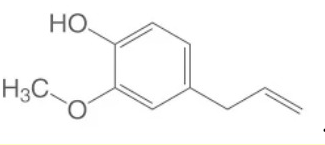
\includegraphics[width=0.32\textwidth]{images_crop_hoa11_de14/eugenol_structure.png}
\end{center}
Cho các phát biểu sau:
\choiceTF
{\True Eugenol tác dụng được với Na và \ce{NaOH} theo tỉ lệ mol 1:1}
{\True Eugenol không có đồng phân hình học}
{\True Hydrogen hoá hoàn toàn eugenol, thu được sản phẩm hữu cơ có tên gọi là 2-methoxy-4-propylcyclohexanol (nhóm methoxy có công thức là \ce{CH3O-})}
{Eugenol có tính acid mạnh}
\loigiai{
- a) ĐÚNG: Phân tử eugenol chứa 1 nhóm \ce{-OH} phenol nên phản ứng được với cả Na và dung dịch \ce{NaOH} theo tỉ lệ mol 1:1. Nhóm ether \ce{-OCH3} và liên kết đôi \ce{C=C} không tác dụng với \ce{NaOH}.\\
- b) ĐÚNG: Nhóm allyl \ce{-CH2-CH=CH2} có carbon nối đôi ở đầu mạch chứa 2 nguyên tử H giống nhau (\ce{=CH2}) nên không có đồng phân hình học cis-trans.\\
- c) ĐÚNG: Khi hydrogen hóa hoàn toàn, liên kết đôi \ce{C=C} ở nhánh allyl và vòng benzene đều bị hydrogen hóa hoàn toàn thành vòng cyclohexane no và nhóm propyl, sản phẩm thu được là 2-methoxy-4-propylcyclohexanol.\\
- d) SAI: Eugenol chứa nhóm \ce{-OH} phenol nên có tính acid rất yếu (không làm đổi màu quỳ tím, yếu hơn cả carbonic acid), không phải acid mạnh.
}
\end{ex}

\bigskip
\noindent\textbf{\large PHẦN III. Câu trắc nghiệm yêu cầu trả lời ngắn.}
\textit{Thí sinh trả lời từ câu 1 đến câu 6.}
\vspace{0.2cm}

% Câu 1 Phần III
\begin{ex}
Cho công thức khung phân tử của hợp chất X như hình dưới đây:
\begin{center}
	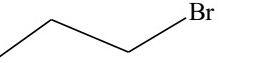
\includegraphics[width=0.3\textwidth]{images_crop_hoa11_de14/propane_br_structure.png}
\end{center}
Nguyên tử Br gắn vào nguyên tử carbon ở vị trí số mấy?
\loigiai{
Mạch chính có 3 carbon: $\overset{3}{\text{C}}\text{H}_3 - \overset{2}{\text{C}}\text{H}_2 - \overset{1}{\text{C}}\text{H}_2 - \text{Br}$.\\
Đánh số mạch carbon ưu tiên từ đầu gần nhóm thế Br nhất, do đó nguyên tử Br gắn vào carbon ở vị trí số 1 (1-bromopropane).\\
$\Rightarrow$ Đáp số: \textbf{1}.
}
\end{ex}

% Câu 2 Phần III
\begin{ex}
Chloromethane được hình thành từ methane và chlorine theo phản ứng sau:
\[ \ce{CH4 + 3Cl2 ->[asmt] CHCl3 + 3HCl} \quad (1) \]
Cho nhiệt tạo thành chuẩn của một chất tương ứng trong phương trình như sau:
\begin{center}
\begin{tabular}{|l|c|c|c|}
\hline
\textbf{Chất} & \ce{CH4(g)} & \ce{CHCl3(g)} & \ce{HCl(g)} \\
\hline
$\Delta_f H^\circ_{298}$ (kJ/mol) & $-75$ & $-103$ & $-92$ \\
\hline
\end{tabular}
\end{center}
Biến thiên enthalpy chuẩn của phản ứng (1) bằng bao nhiêu kJ?
\loigiai{
Áp dụng công thức tính biến thiên enthalpy chuẩn từ nhiệt tạo thành:
\[ \Delta_r H^\circ_{298} = \Delta_f H^\circ_{298}(\ce{CHCl3}(g)) + 3 \times \Delta_f H^\circ_{298}(\ce{HCl}(g)) - \Delta_f H^\circ_{298}(\ce{CH4}(g)) \]
\[ \Delta_r H^\circ_{298} = -103 + 3 \times (-92) - (-75) = -103 - 276 + 75 = -304\text{ kJ}. \]
$\Rightarrow$ Đáp số: \textbf{-304}.
}
\end{ex}

% Câu 3 Phần III
\begin{ex}
Cho các chất sau: (1) Dung dịch \ce{HCl} đặc; (2) Dung dịch \ce{Cu(OH)2}; (3) Nước bromine; (4) Dung dịch \ce{H2SO4} đặc, nóng; (5) Na; (6) \ce{CuO} ($t^\circ$, xt); (7) \ce{CH3COOH}; (8) \ce{O2} ($t^\circ$). Có bao nhiêu chất tác dụng được với ethyl alcohol?
\loigiai{
Ethyl alcohol (\ce{C2H5OH}) tác dụng được với 6 chất:
\begin{itemize}
    \item (1) Dung dịch \ce{HCl} đặc: \ce{C2H5OH + HCl ->[{t$^\circ$}] C2H5Cl + H2O}.
    \item (4) Dung dịch \ce{H2SO4} đặc, nóng (tách nước tạo \ce{C2H4} hoặc \ce{(C2H5)2O}).
    \item (5) Na: \ce{2C2H5OH + 2Na -> 2C2H5ONa + H2}.
    \item (6) \ce{CuO} ($t^\circ$): \ce{C2H5OH + CuO ->[{t$^\circ$}] CH3CHO + Cu + H2O}.
    \item (7) \ce{CH3COOH} (phản ứng ester hóa với xúc tác \ce{H2SO4} đặc).
    \item (8) \ce{O2} ($t^\circ$): phản ứng cháy tạo \ce{CO2} và \ce{H2O}.
\end{itemize}
Không tác dụng với: (2) Dung dịch \ce{Cu(OH)2}; (3) Nước bromine.\\
$\Rightarrow$ Đáp số: \textbf{6}.
}
\end{ex}

% Câu 4 Phần III
\begin{ex}
Cho dãy các chất/dung dịch sau: \ce{NaOH}, \ce{NaHCO3}, \ce{HCl}, \ce{NaNO3}, nước \ce{Br2} phản ứng với phenol. Có bao nhiêu chất phản ứng với phenol?
\loigiai{
Phenol (\ce{C6H5OH}) có tính acid yếu và phản ứng thế nhân thơm:
\begin{itemize}
    \item Tác dụng với dung dịch \ce{NaOH}: \ce{C6H5OH + NaOH -> C6H5ONa + H2O}.
    \item Tác dụng với dung dịch nước bromine (\ce{Br2}): \ce{C6H5OH + 3Br2 -> C6H2Br3OH v} (trắng) \ce{+ 3HBr}.
\end{itemize}
Phenol không phản ứng với \ce{NaHCO3} (do tính acid yếu hơn \ce{H2CO3}), \ce{HCl} và \ce{NaNO3}.\\
$\Rightarrow$ Đáp số: \textbf{2}.
}
\end{ex}

% Câu 5 Phần III
\begin{ex}
Hợp chất X có tên 3,5-dibromo-8,8-dichloro-2,6-dimethyl-1,6-octadiene là một dẫn xuất halogen tách ra từ biển đỏ chi Laurencia có tác dụng chống ung thư vòm họng. Biết rằng X có chứa 4 nguyên tố với thành phần khối lượng như sau: 32,88\% C; 3,84\% H; 43,84\% Br; còn lại là chlorine. Biết rằng trong X có chứa hai nguyên tử chlorine. Số nguyên tử C trong phân tử X là bao nhiêu?
\loigiai{
Thành phần phần trăm khối lượng của chlorine trong X:
\[ \%Cl = 100\% - (32{,}88\% + 3{,}84\% + 43{,}84\%) = 19{,}44\%. \]
Vì phân tử X chứa 2 nguyên tử chlorine:
\[ M_X = \frac{2 \times 35{,}5}{19{,}44\%} \approx 365{,}23\text{ g/mol}. \]
Số nguyên tử C trong phân tử X là:
\[ n_C = \frac{365{,}23 \times 32{,}88\%}{12} \approx 10. \]
$\Rightarrow$ Đáp số: \textbf{10}.
}
\end{ex}

% Câu 6 Phần III
\begin{ex}
Củ sắn khô chứa 38\% khối lượng là tinh bột, còn lại là các chất không có khả năng lên men thành ethyl alcohol. Xăng E5 có 5\% thể tích là ethyl alcohol. Dùng toàn bộ lượng ethyl alcohol thu được ở trên để pha chế xăng E5. Tính thể tích xăng E5 thu được sau khi pha trộn (theo lít), biết khối lượng riêng của ethyl alcohol là 0,8 kg/L, hiệu suất của cả quá trình lên men từ tinh bột là 81\%, lấy 1 tấn củ sắn khô làm nguyên liệu.
\loigiai{
Khối lượng củ sắn khô: $m = 1\text{ tấn} = 1000\text{ kg}$.\\
Khối lượng tinh bột: $m_{\text{tinh bột}} = 1000 \times 38\% = 380\text{ kg}$.\\
Sơ đồ phản ứng lên men:
\[ \ce{(C6H10O5)_n ->[{+n H_2O}] n C6H12O6 ->[{men}] 2n C2H5OH + 2n CO2} \]
Theo lí thuyết: $162\text{ kg tinh bột} \to 92\text{ kg \ce{C2H5OH}}$.\\
Khối lượng \ce{C2H5OH} thực tế thu được với $H = 81\%$:
\[ m_{\text{ethanol}} = \frac{380 \times 92}{162} \times 81\% = 174{,}8\text{ kg}. \]
Thể tích ethyl alcohol thu được:
\[ V_{\text{ethanol}} = \frac{m}{D} = \frac{174{,}8}{0{,}8} = 218{,}5\text{ lít}. \]
Vì ethyl alcohol chiếm 5\% thể tích xăng E5, nên thể tích xăng E5 thu được là:
\[ V_{\text{xăng}} = \frac{218{,}5}{5\%} = \frac{218{,}5 \times 100}{5} = 4370\text{ lít}. \]
$\Rightarrow$ Đáp số: \textbf{4370}.
}
\end{ex}

\bigskip
\noindent\textbf{\large PHẦN IV. Câu hỏi tự luận.}
\textit{Thí sinh trình bày lời giải chi tiết vào giấy làm bài.}
\vspace{0.2cm}

% Câu 1 Phần IV
\begin{ex}
Tìm thông tin thích hợp điền vào chỗ trống trong mỗi phát biểu sau:
\begin{enumerate}[a)]
    \item Propane-1,2,3-triol có tên thông thường là \dotfill
    \item Cho ethane-1,2-diol vào ống nghiệm có \ce{Cu(OH)2} và dung dịch \ce{NaOH}, lắc nhẹ, hiện tượng quan sát được là \dotfill
    \item Đun nóng hỗn hợp gồm ethanol, methanol và \ce{H2SO4} đặc thu được tối đa ....(1)...... ether có công thức cấu tạo là .....(2).....
    \item Cho $a$ mol alcohol \ce{R(OH)_n} phản ứng với Na (dư) thu được tối đa $a$ mol khí \ce{H2}. Giá trị của $n$ là \dotfill
\end{enumerate}

\loigiai{
a) glycerol (hoặc glixerin).\\
b) kết tủa tan, tạo dung dịch màu xanh lam đậm.\\
c) (1) : 3\\
\hspace*{0.5cm} (2) : \ce{CH3-O-CH3} ; \ce{C2H5-O-C2H5} ; \ce{CH3-O-C2H5}.\\
d) Phản ứng: \ce{R(OH)_n + n Na -> R(ONa)_n + \frac{n}{2} H2}.\\
Theo phương trình: $n_{\ce{H2}} = \frac{n}{2} \times n_{\text{alcohol}} \iff a = \frac{n}{2} \times a \Rightarrow \frac{n}{2} = 1 \Rightarrow n = 2$.\\
Giá trị của $n$ là 2.
}

\end{ex}

% Câu 2 Phần IV
\begin{ex}
(SBT-CD) Hợp chất A là dẫn xuất monochloro của alkylbenzene (B). Phân tử khối của A bằng 126,5.
\begin{enumerate}[a)]
    \item Tìm công thức phân tử và viết công thức cấu tạo có thể có của A.
    \item Chất A có phản ứng thuỷ phân khi đun nóng với dung dịch \ce{NaOH}, tạo ra chất E có mùi thơm, có khả năng hoà tan nhiều chất hữu cơ, ức chế sự sinh sản của vi khuẩn nên được dùng nhiều trong công nghiệp sản xuất mỹ phẩm. Tìm công thức cấu tạo đúng của A. Viết phương trình hoá học của phản ứng.
    \item Viết phương trình hoá học của phản ứng điều chế trực tiếp A từ B, ghi rõ điều kiện của phản ứng.
\end{enumerate}

\loigiai{
a) A là dẫn xuất monochloro của alkylbenzene nên công thức có dạng \ce{C_nH_{2n-7}Cl} ($n \ge 7$).\\
Phân tử khối: $M_A = 14n + 28{,}5 = 126{,}5 \Rightarrow 14n = 98 \Rightarrow n = 7$.\\
Công thức phân tử của A là \ce{C7H7Cl}.\\
Các công thức cấu tạo có thể có của A gồm 4 đồng phân:
\begin{itemize}
    \item (1) 2-chlorotoluene (\textit{o}-chlorotoluene): \ce{\textit{o}-CH3-C6H4-Cl}
    \item (2) 3-chlorotoluene (\textit{m}-chlorotoluene): \ce{\textit{m}-CH3-C6H4-Cl}
    \item (3) 4-chlorotoluene (\textit{p}-chlorotoluene): \ce{\textit{p}-CH3-C6H4-Cl}
    \item (4) benzyl chloride: \ce{C6H5CH2Cl}.
\end{itemize}
\begin{center}
	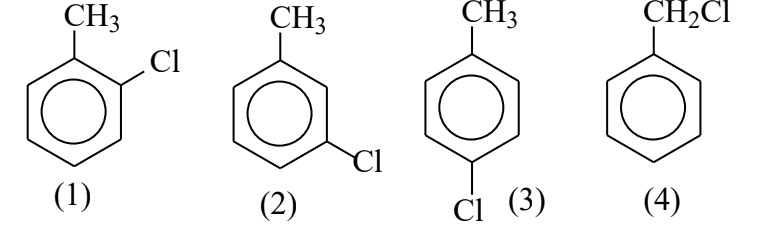
\includegraphics[width=0.65\textwidth]{images_crop_hoa11_de14/monochloro_isomers.png}
\end{center}
b) Các đồng phân (1), (2), (3) có nguyên tử Cl liên kết trực tiếp với vòng benzene rất bền, không bị thủy phân bởi dung dịch \ce{NaOH} đun nóng ở điều kiện thường.\\
Chỉ có đồng phân (4) benzyl chloride (\ce{C6H5CH2Cl}) có nguyên tử Cl ở mạch nhánh dễ dàng bị thủy phân tạo benzyl alcohol (E):\\
\ce{C6H5CH2Cl + NaOH ->[{t$^\circ$}] C6H5CH2OH + NaCl}.\\
Benzyl alcohol (E) là chất lỏng có mùi thơm dịu, kháng khuẩn, dùng trong sản xuất mỹ phẩm.\\
Vậy công thức cấu tạo đúng của A là (4): \ce{C6H5CH2Cl} (benzyl chloride).\\
c) Alkylbenzene B là toluene (\ce{C6H5CH3}). Điều chế trực tiếp benzyl chloride (A) từ toluene bằng phản ứng clo hóa nhánh với ánh sáng:\\
\ce{C6H5CH3 + Cl2 ->[as] C6H5CH2Cl + HCl}.
}

\end{ex}

\newpage
\noindent\textbf{\large BẢNG ĐÁP ÁN THAM KHẢO PHẦN I}
\vspace{0.2cm}

\begin{center}
\begin{tabular}{|c|c|c|c|c|c|c|c|c|}
\hline
\textbf{1. C} & \textbf{2. B} & \textbf{3. B} & \textbf{4. B} & \textbf{5. A} & \textbf{6. B} & \textbf{7. B} & \textbf{8. A} & \textbf{9. B} \\
\hline
\textbf{10. C} & \textbf{11. C} & \textbf{12. B} & \textbf{13. D} & \textbf{14. B} & \textbf{15. C} & \textbf{16. B} & \textbf{17. A} & \textbf{18. A} \\
\hline
\end{tabular}
\end{center}

\bigskip
\noindent\textbf{\large BẢNG ĐÁP ÁN THAM KHẢO PHẦN II}
\vspace{0.2cm}

\begin{center}
\begin{tabular}{|c|c|c|c|c|}
\hline
\textbf{Câu} & \textbf{Ý a)} & \textbf{Ý b)} & \textbf{Ý c)} & \textbf{Ý d)} \\
\hline
\textbf{Câu 1} & Đ & Đ & S & Đ \\
\hline
\textbf{Câu 2} & S & S & Đ & S \\
\hline
\textbf{Câu 3} & Đ & S & Đ & S \\
\hline
\textbf{Câu 4} & Đ & Đ & Đ & S \\
\hline
\end{tabular}
\end{center}

\bigskip
\noindent\textbf{\large BẢNG ĐÁP ÁN THAM KHẢO PHẦN III}
\vspace{0.2cm}

\begin{center}
\begin{tabular}{|c|c|c|c|c|c|}
\hline
\textbf{Câu 1} & \textbf{Câu 2} & \textbf{Câu 3} & \textbf{Câu 4} & \textbf{Câu 5} & \textbf{Câu 6} \\
\hline
1 & -304 & 6 & 2 & 10 & 4370 \\
\hline
\end{tabular}
\end{center}

\begin{center}
\textbf{--------- HẾT ---------}
\end{center}

\end{document}
